% Document class
\documentclass[12pt]{article}

% Packages
\usepackage[margin=1in]{geometry}
\usepackage{setspace}
\usepackage{amsmath}
\usepackage{graphicx}
\usepackage{booktabs}
\usepackage{caption}
\usepackage{subcaption}
\usepackage{natbib}
\usepackage{hyperref}
\usepackage{float}
\usepackage{xcolor}

% Document settings
\doublespacing
\setlength{\parskip}{6pt}
\setlength{\parindent}{0.5in}

\begin{document}

\begin{titlepage}
    \begin{center}
        \vspace*{1cm}
        
        \Huge
        \textbf{Does Level of Assurance Service Impact Financial Institution Failure?}
        
        \vspace{0.5cm}
        \LARGE
        A Study of Assurance Services and Community Bank Behavior
        
        \vspace{1.5cm}
        
        \vfill
        
        \Large
        Laura Wardwell\\ 
        ECON5253\\
        \today
    \end{center}
\end{titlepage}

\section{Introduction}

Community banks represent 96\% of all the nearly 5,000 banks in the United States as of 2022 \citep{KandracMarsh2025}. These institutions fill important gaps in the banking system, especially for small business, agricultural, and rural customers \citep{ICBA2024, KandracMarsh2025}. Community bank managers in the United States routinely grapple with competing priorities from regulators and shareholders. Managers at these institutions must balance expensive regulatory oversight with expense control to avoid erosion of shareholder returns and required capital \citep{KandracMarsh2025}.

One such regulatory aspect is the requirement for financial statement audits and internal control audits. To provide relief for small banks, U.S. banking regulation has developed a tiered system, which offers some measures of relief to smaller institutions with less ability to bear monitoring costs. One such concession grants community banks under \$500 million assets an exemption from the requirement for a financial statement audit, and banks under \$1 billion an exemption from the requirement for an integrated audit of internal controls \citep{Jin2013a, Jin2013b}. This tiered system creates a unique setting where we can investigate whether distinct levels of assurance services affect community bank failure rates.

The failure of community banks can have particularly devastating effects on local communities. Unlike larger institutions with geographically diverse operations, when a community bank fails, it can creates gaps in financial services for the local area. Community bank failure can disrupt established lending relationships, reduce credit availability, and disrupt the institutional knowledge about local economic conditions that these banks accumulate over time. This disruption is particularly acute in rural and underserved areas where community banks may be the only financial institution in operation.

Understanding the relationship between the level of financial statement assurance obtained by community bank management and bank failure is therefore important for multiple reasons. First, the community bank setting offers a rare opportunity to study different assurance levels that are typically unobservable in other small, privately owned company contexts. Second, if higher assurance levels correlate with lower failure rates, this study would provide empirical evidence to inform bank management decisions when reviewing the cost-benefit analysis for obtaining assurance services. Finally, regulatory outcomes may be influenced by the presence of higher levels of assurance, as the FDIC considers the quality of internal control a key ``Management'' evaluation factor in the Uniform Financial Institutions Rating System \citep{FDIC2023}.

\section{Literature Review}

\subsection{Community Banking in the United States}

The United States banking industry has diverged into two distinct models. The largest banks operating regional, national, or international networks have increased market share during the last three decades and possess high systemic threat to the banking system in the event of failure, a phenomenon often referred to as ``too big to fail''. The second group of smaller banks, referred to as community banks, focuses on local operations and gains information advantages from deeper relationships within a smaller geographic area \citep{KandracMarsh2025}.

Community banks generally focus on relationship banking and can apply more discretionary judgments when working with customers, as opposed to bright line customer criteria, such as credit scores and minimum metrics, often utilized by larger institutions \citep{ICBA2024}. In a survey of small businesses conducted in 2022, the Federal Reserve found business lending applicants at small banks were more satisfied with their experience, over those who received funding from large banks, finance companies, and online lenders \citep{FRB2023}, suggesting better relationships between community bank lenders and their borrowing customers. These strong relationships between a borrower and financial institution are particularly useful in times of crisis or economic downturn.

\citet{KandracMarsh2025} also note that while community banks held a small percentage (15\%) of all bank loans as of 2019, these institutions held a larger portion of small business loans (36\%) in the same year. This is consistent with community banking institutions fulfilling a significant role in local markets and benefiting from reduced information asymmetry between the institution and borrower. A community bank lender can access more information through the closer local relationship and provide access to financial services which might be denied by a larger institution.

Community banks are particularly important to rural communities, where more complex agricultural lending needs are higher and fewer deposit services are present. Relationship lending at community banks offers superior information processing for agricultural borrowers, who function in a highly specialized industry with uniquely local conditions \citep{KandracMarsh2025}. Community banks also fulfill an important need for in-person deposit services in rural areas. In 2015, rural communities had an unbanked population of 7.6\% \citep{HayashiMinhas2018}, representing individuals at high risk for usurious financial fees. Unbanked individuals are often subjected to higher cost Alternative Financial Services, which erode income directly through additional fees for services such as check-cashing and funds transfer, and high-interest refund anticipation loans, and indirectly through a lack of access to wealth-building savings products \citep{Barr2004}.

\subsection{Community Bank Regulation}

In the United States, modern financial regulation developed mostly as a series of responses to serious financial crises, with each crisis from the Great Depression to the early 2000's financial crisis prompting significant revisions to monitoring and oversight processes \citep{KandracMarsh2025}. One such response to a crisis, the Financial Institutions Reform, Recovery and Enforcement Act (FIRREA) of 1989, marked a significant regulatory shift following the Savings and Loan Crisis (also called the ``Thrift Crisis'') of the 1980's. During the heart of the crisis, over 500 institutions specifically designated as savings institutions failed, exceeding the total of the previous four decades combined \citep{Clark1989}.

As FIRREA's provisions expanded regulatory authority to monitor financial institution health, the Federal Deposit Insurance Corporation (FDIC) expanded the information requirements of quarterly Reports of Condition and Income, also known as Call Reports, to include information on the level of financial statement assurance provided by external accountants. This creates a unique setting where we investigate whether the level of assurance affects community bank outcomes, specifically focusing on failure rates.

The FIRREA was followed by the Federal Deposit Insurance Corporation Improvement Act (FDICIA) in 1991, which further required banks over \$500 million in assets (adjusted to \$1 billion in assets in 2005) to receive an integrated audit of both the institution financial statements and the internal controls over financial reporting \citep{Akhigbe2001, Jin2013b}. The implementation of stratified FDICIA rules and the subsequent change in the FDICIA asset threshold separates community banks into three different groups after 2005: one group above the \$1 billion asset threshold for whom the highest level of audit assurance is mandatory, one group between the \$500 million and \$1 billion asset threshold for whom at least financial statement audit is required, and a final group below the \$500 million threshold with the ability to choose the preferred level of assurance service, which may include no assurance, absent regulatory intervention.

\subsection{The Role of Assurance in Community Banking}

According to agency theory, monitoring activities necessarily restrain manager behavior and reduce agency costs related to opportunistic manager behavior \citep{JensenMeckling1976}. However, community bank managers operate in an environment with pre-existing high regulatory monitoring, and when choosing to engage an independent third party, must select external monitoring services based on a cost and benefit tradeoff. For the smallest community banks, the highest levels of assurance service may not contain enough incremental benefit to the organization to justify the expenditure of capital \citep{AbdelKhalik1993}.

Differing levels of assurance may provide different signals to financial statement users regarding firm type \citep{Dharan1992}, in addition to any operational benefits to the firm. Prior research has demonstrated that audit quality can impact financial reporting quality in the banking industry \citep{Beck2022}, which may in turn affect regulatory oversight and bank stability. \citet{Ege2025} find that increased auditor scrutiny of loan loss provisions can affect bank lending practices, suggesting that higher assurance levels might influence key risk areas that relate to bank failure.

Higher levels of assurance may also assist regulatory agencies and increase examiner efficiency in the process of evaluating safety and soundness. Using proprietary bank examination data obtained from the Federal Reserve Bank of St. Louis, \citet{Gopalan2024} found regulators appear to rely on higher levels of assurance services during the examination process. This study found that for banks who were no longer subject to FDICIA internal controls requirements and no longer obtained an ICFR audit after the 2005 change in asset size threshold, the average length of a targeted examination increased by 9.8 days, which is consistent with greater regulator effort after a decrease in level of external audit assurance.

In a study of PCAOB inspected auditors, \citet{StuberHogan2021} found bank estimates of the allowance for loan loss became more conservative after periods of higher PCAOB scrutiny of ALL substantive testing. Concern for litigation risk can also influence auditor assessment at banks, as auditors increase conservatism at surviving clients after experiencing the failure of another bank client \citep{Hall2023}.

\section{Hypothesis Development}

In the high regulation environment of community banks, it is possible financial statement audit or integrated audits including an opinion of internal control over financial reporting may have little incremental value over regulatory monitoring. However, as shown by prior research on the influence of audit assurance on bank behavior \citep{Jin2013a, Jin2013b, Gopalan2024}, we expect that higher levels of assurance are associated with improved bank stability.

For this study, we focus on the relationship between audit assurance and bank failure rates, leading to our main hypothesis:

\begin{quote}
\textbf{H1:} Higher assurance levels are associated with fewer bank failures at community banks not subject to mandatory audit.
\end{quote}

For banks between \$500 million and \$1 billion in assets that are required to have a financial statement audit but not an integrated audit, we examine whether the choice to obtain an integrated audit is associated with lower failure rates:

\begin{quote}
\textbf{H2:} Receipt of a voluntary integrated audit is associated with fewer bank failures than for community banks receiving a financial statement only audit.
\end{quote}

\section{Data}

\subsection{Data Sources}

This study uses multiple data sources to investigate the relationship between assurance levels and bank failure rates. The primary sources include:

\begin{enumerate}
    \item \textbf{FDIC Call Reports:} Quarterly financial data for US banks from 2000-2023, obtained from the FDIC Statistics on Depository Institutions (SDI) BankFind Suite and the Bank Regulatory Database from Wharton Research Data Services (WRDS). Call reports provide comprehensive financial information, including balance sheet items, income statement details, and regulatory ratios.
    
    \item \textbf{Audit Type Data:} Information on the level of assurance services received by each bank, indicated by the RCON6724 field from March Call Reports (which reports the audit type for the previous year). Following \citet{Douglass2016}, we classify bank assurance levels from 2000$-$2015 into four groups: Audit, Agreed-Upon Procedures, Review \& Compilation, or No Assurance. For the period from 2016$-$2023, we classify bank assurance levels into five groups: Integrated Audit, Financial Statement Only Audit, Agreed-Upon Procedures, Review \& Compilation, or No Assurance.
    
    \item \textbf{FDIC Failed Bank List:} Historical record of bank failures obtained from the FDIC website, covering the period 2001$-$2023. This list provides information on banks that were closed by regulators, including the date of failure and the acquiring institution (if applicable).
\end{enumerate}

\subsection{Sample Selection}

Our initial sample consists of all FDIC-insured commercial banks in the United States from 2000 to 2023. We divided this sample into two subsamples based on asset size:

\begin{enumerate}
    \item \textbf{Small Banks:} Banks with total assets less than \$500 million, for whom audits are not mandatory.
    
    \item \textbf{Medium Banks:} Banks with total assets between \$500 million and \$1 billion, for whom financial statement audits are mandatory but integrated audits are optional.
\end{enumerate}

Our total sample consists of 102,522 bank-year observations for small banks and 8,555 bank-year observations for medium banks. Figure \ref{fig:bank_failures} shows the distribution of bank failures by year for both small and medium-sized banks, highlighting the significant spike in failures during the 2008$-$2010 financial crisis period.

\subsection{Variable Definitions}

The main variables used in our analysis are defined as follows:

\begin{enumerate}
    \item \textbf{Dependent Variable:}
    \begin{itemize}
        \item \textbf{Failure\_t+1:} A binary indicator equal to 1 if the bank failed in year t+1, and 0 otherwise.
    \end{itemize}
    
    \item \textbf{Key Independent Variables:}
    \begin{itemize}
        \item \textbf{Audit:} A binary indicator equal to 1 if the bank received any kind of audit in year t, and 0 otherwise.
        \item \textbf{Integrated:} A binary indicator equal to 1 if the bank received an integrated audit in year t (only available post-2016), and 0 otherwise.
        \item \textbf{FSOnly:} A binary indicator equal to 1 if the bank received a financial statement-only audit in year t (only available post-2016), and 0 otherwise.
    \end{itemize}
    
    \item \textbf{Control Variables:}
    \begin{itemize}
        \item \textbf{Size:} Natural log of total assets.
        \item \textbf{Charge-offs:} Net charge-offs to total loans ratio.
        \item \textbf{NPA:} Non-performing assets ratio, calculated as the sum of loans past due 30-89 days, loans past due 90+ days, and non-accrual loans divided by total loans.
        \item \textbf{CommRE:} Commercial real estate concentration, calculated as commercial real estate loans divided by total net loans.
        \item \textbf{Mortgage:} Mortgage concentration, calculated as total mortgage loans divided by total net loans.
        \item \textbf{C\&I:} Commercial and industrial concentration, calculated as total commercial and industrial loans divided by total net loans.
        \item \textbf{Consumer:} Consumer loan concentration, calculated as total consumer loans divided by total net loans.
        \item \textbf{Capital:} Tier 1 capital ratio.
        \item \textbf{ALL:} Allowance for loan and lease losses to total loans ratio.
        \item \textbf{BR\_Ratio:} Brokered deposits ratio, calculated as total brokered deposits divided by total deposits.
        \item \textbf{SubchapterS:} Binary indicator for banks with Subchapter S tax status.
    \end{itemize}
\end{enumerate}

\subsection{Descriptive Statistics}

Tables \ref{tab:stats_small} and \ref{tab:stats_medium} present the descriptive statistics for our sample of small banks and medium-sized banks, respectively.

\section{Methods}

\subsection{Model Specification}

To test our hypotheses about the relationship between audit assurance levels and bank failure, we employ a logistic regression model. The binary nature of our dependent variable (bank failure) makes logistic regression an appropriate choice for this analysis. Our main model specification is:

$$\Pr(Failure_{i,t+1}) = \beta_0 + \beta_1 Audit_{i,t} + \beta_2 Size_{i,t} + \beta_3 Controls_{i,t} + \gamma_t + \delta_j + \epsilon_{i,t}$$

Where:

\begin{itemize}
    \item $Failure_{i,t+1}$ is a binary indicator for bank failure in period t+1
    \item $Audit_{i,t}$ is our key independent variable indicating the type of audit received in period t
    \item $Size_{i,t}$ is the natural log of total assets
    \item $Controls_{i,t}$ represents our vector of control variables
    \item $\gamma_t$ represents year fixed effects
    \item $\delta_j$ represents Federal Reserve district fixed effects
    \item $\epsilon_{i,t}$ is the error term
\end{itemize}

For small banks (assets $<$ \$500 million), the key independent variable is the binary indicator for whether the bank received any kind of audit. For medium banks (assets between \$500 million and \$1 billion), we use separate indicators for integrated audit and financial statement-only audit in the later period (2016-2023).

All models include year fixed effects to control for macroeconomic conditions and Federal Reserve district fixed effects to account for regional variation in regulatory approach and economic conditions. We estimate our models with robust standard errors clustered at the bank level to account for potential serial correlation in the error terms.

\subsection{Empirical Strategy}

To address potential endogeneity concerns related to the bank's choice to pursue higher levels of assurance, we include a comprehensive set of control variables that capture bank financial health, risk profile, and business model. These controls help mitigate concerns that omitted variables might drive both the decision to obtain higher levels of assurance and the probability of bank failure.

We run separate regressions for the two bank size categories:

\begin{enumerate}
    \item For small banks ($<$ \$500 million), we test whether receiving any audit is associated with lower failure rates compared to lower levels of assurance or no assurance.
    
    \item For medium banks (\$500 million $-$ \$1 billion), we test whether receiving an integrated audit is associated with lower failure rates compared to receiving only a financial statement audit.
\end{enumerate}

We report our results in terms of both logistic regression coefficients and marginal effects to facilitate interpretation.

\section{Findings}

\subsection{Regression Results}

Table 3 presents the logistic regression results for both small banks (assets $<$ \$500 million) and medium-sized banks (assets between \$500 million and \$1 billion). The dependent variable in all models is bank failure in period t+1.

For small banks, the coefficient on the Audit variable is negative and statistically significant at the 5\% level (coefficient = -0.563, p $<$ 0.05). This suggests that receiving an audit is associated with a lower probability of failure in the following year, supporting our first hypothesis (H1). The economic significance of this effect is substantial, indicating that small banks that receive an audit have a lower probability of failure compared to those that do not, after controlling for other factors.

For medium-sized banks, the coefficient on the Integrated Audit variable is negative but not statistically significant (coefficient = -0.290, p $>$ 0.10). This suggests that receiving an integrated audit, as compared to only a financial statement audit, is not significantly associated with a lower probability of failure in the following year. Therefore, we do not find statistical support for our second hypothesis (H2). During the period examined, the COVID-19 pandemic prompted serious regulatory relief measures, particularly aimed at community banks to facilitate the distribution of funds to small business via the Paycheck Protection Program (PPP). Community banks were instrumental in the distribution of funds from the PPP to small businesses, and regulatory capital requirements were relaxed to ensure community banks did not feel disincentivized to participate in the program. These capital concessions may contribute to regulatory forbearance during 2020 $-$ 2022, and therefore distort the statistical analysis.

Regarding control variables, we find that bank size (Size) is negatively associated with failure probability for both small and medium-sized banks, suggesting that larger banks within each size category are less likely to fail. The non-performing assets ratio (NPA) is positively associated with failure probability, consistent with the intuition that banks with more problem loans are at higher risk of failure. Consumer loan concentration (Consumer) is negatively associated with failure probability, suggesting that banks with higher consumer loan concentrations are less likely to fail. For medium-sized banks, mortgage concentration (Mortgage) is negatively associated with failure probability, while commercial and industrial loan concentration (ComInd) is positively associated with failure probability.

The Tier 1 capital ratio (Capital) is strongly negatively associated with failure probability for small banks, which aligns with the regulatory emphasis on capital adequacy as a safeguard against failure. For small banks, the brokered deposits ratio (BR\_Ratio) is positively associated with failure probability, consistent with the view that reliance on brokered deposits may indicate funding instability.

\section{Conclusion}

This study examines whether the level of assurance service impacts financial institution stability, specifically focusing on bank failure rates. We find evidence that for small community banks (assets $<$ \$500 million), higher assurance levels in the form of financial statement audits are associated with lower probability of failure in the following year. This finding supports the view that external audits provide an important monitoring function that complements regulatory oversight and potentially improves bank stability.

For medium-sized community banks (assets \$500 million $-$ \$1 billion), we do not find statistically significant evidence that integrated audits of internal controls over financial reporting provide incremental benefits over financial statement-only audits in terms of reducing failure probability. However, this result should be interpreted with caution due to the smaller sample size and relatively few failures in the post-2016 period, which may be due in part to regulator forbearance during the COVID-19 pandemic. Unfortunately, the presence of complex economic issues during the 2020 $-$ 2022 period may distort the integrated audit analysis.

\subsection{Implications}

Our findings have several important implications:

\begin{enumerate}
    \item \textbf{Policy considerations:} The current regulatory thresholds for mandatory audit requirements appear to have some merit, as small banks that voluntarily adopt higher assurance levels exhibit lower failure rates. This suggests that regulators should carefully consider the potential impacts before raising the threshold for integrated audit requirements as proposed by industry groups like the ICBA.
    
    \item \textbf{Early warning signals:} Changes in audit type may signal changing risk profiles at banks. Regulators and stakeholders might benefit from monitoring not just financial metrics but also changes in the level of assurance services chosen by banks.
    
    \item \textbf{Cost-benefit analysis for bank management:} Our results suggest that for small banks, the benefits of obtaining an audit may include reduced failure risk, which should be considered when banks evaluate the costs of assurance services.
\end{enumerate}

\subsection{Limitations and Future Research}

This study has several limitations that suggest directions for future research:

First, the choice to obtain a financial statement audit or an integrated audit when not explicitly required by regulation may be related to other unobservable factors such as corporate governance quality or primary regulator activities. While we control for observable bank characteristics, there may be omitted variables that influence both the decision to obtain higher levels of assurance and the probability of failure.

Second, regulation in the banking industry is a continuous process, with intense regulatory examination occurring at least once every 18 months for many banks in the dataset, or more frequently as warranted by a bank's financial condition. Regulators may require banks to obtain audits as part of enforcement actions, which could influence our results.

Overall, this study contributes to the understanding of how external assurance services affect bank stability and provides empirical evidence that can inform both regulatory policy and bank management decisions regarding assurance services.

\clearpage
\begin{figure}[H]
    \centering
    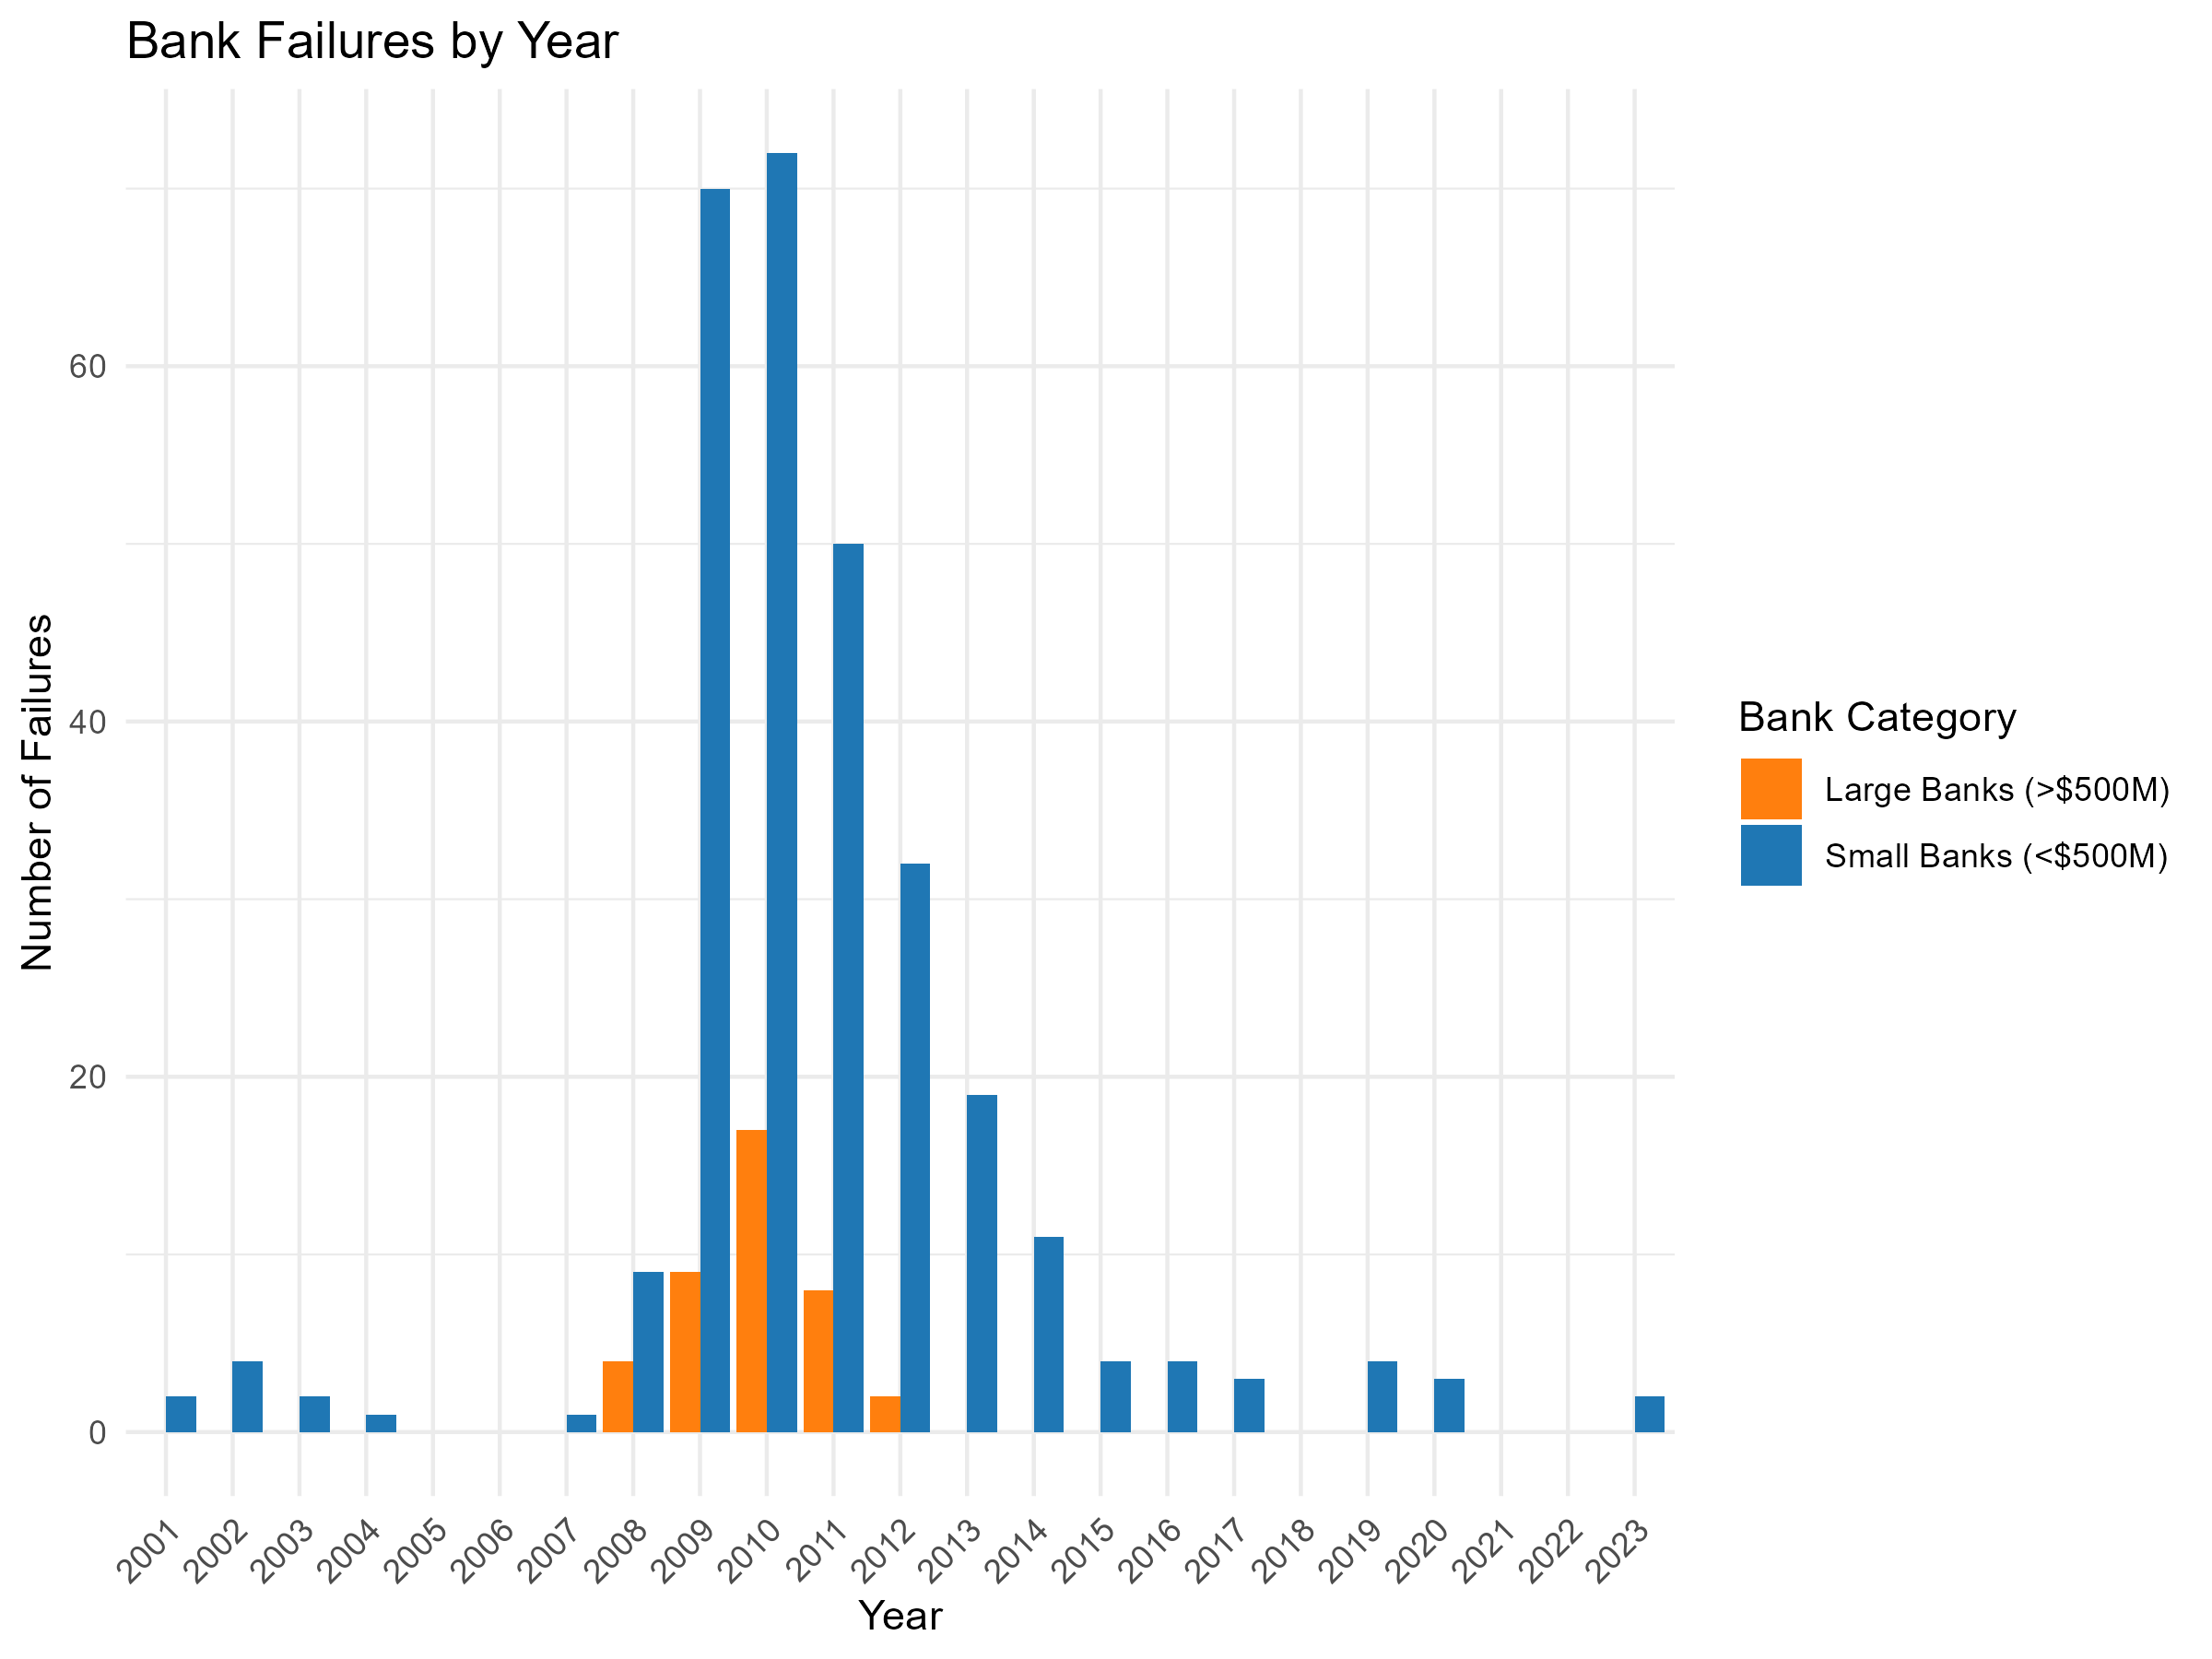
\includegraphics[width=0.9\textwidth]{bank_failures_plot.png}
    \caption{Bank Failures by Year}
    \label{fig:bank_failures}
\end{figure}

\clearpage
\begin{table}[H]
\centering
\caption{Summary Statistics $-$ Banks $<$ 500MM in Assets}
\label{tab:stats_small}
\begin{tabular}{lccccccc}
\toprule
Statistic & Mean & St. Dev. & Min & Pct(25) & Median & Pct(75) & Max \\
\midrule
Failure t+1 & 0.002 & 0.048 & 0 & 0 & 0 & 0 & 1 \\
Audit & 0.611 & 0.488 & 0 & 0 & 1 & 1 & 1 \\
Size & 11.571 & 0.900 & 5.333 & 10.968 & 11.637 & 12.269 & 13.122 \\
Charge Offs & 0.004 & 0.338 & -2.909 & 0.00004 & 0.001 & 0.003 & 120.234 \\
Non-performing Assets & 0.014 & 0.024 & 0.000 & 0.002 & 0.007 & 0.017 & 1.000 \\
Commercial RE & 0.221 & 0.159 & 0.000 & 0.095 & 0.194 & 0.315 & 1.037 \\
Mortgage & 0.300 & 0.203 & 0.000 & 0.153 & 0.263 & 0.401 & 1.270 \\
Comm Ind & 0.143 & 0.115 & 0.000 & 0.072 & 0.121 & 0.188 & 9.333 \\
Consumer & 0.082 & 0.101 & 0.000 & 0.022 & 0.053 & 0.105 & Infinity \\
Capital & 0.209 & 2.115 & -0.135 & 0.116 & 0.145 & 0.194 & 396.933 \\
ALL & 0.015 & 0.012 & 0.000 & 0.010 & 0.013 & 0.017 & 0.893 \\
Brokered Deposits & 0.025 & 0.198 & 0.000 & 0.000 & 0.000 & 0.008 & 66.232 \\
Subchapter S & 0.328 & 0.470 & 0 & 0 & 0 & 1 & 1 \\
\bottomrule
\multicolumn{8}{l}{Sample period: 2000-2022. Federal Reserve Districts: 1, 2, 3, 4, 5, 6, 7, 8, 9, 10, 11, 12.}
\end{tabular}
\end{table}

\begin{table}[H]
\centering
\caption{Summary Statistics $-$ Banks $<$ 1B in Assets}
\label{tab:stats_medium}
\begin{tabular}{lccccccc}
\toprule
Statistic & Mean & St. Dev. & Min & Pct(25) & Median & Pct(75) & Max \\
\midrule
Failure t+1 & 0.0004 & 0.019 & 0 & 0 & 0 & 0 & 1 \\
Audit & 0.608 & 0.488 & 0 & 0 & 1 & 1 & 1 \\
Size & 12.148 & 0.939 & 7.824 & 11.518 & 12.203 & 12.868 & 13.815 \\
Charge Offs & 0.001 & 0.012 & -0.482 & -0.00001 & 0.0002 & 0.001 & 1.352 \\
Non-performing Assets & 0.009 & 0.015 & 0.000 & 0.001 & 0.004 & 0.011 & 0.561 \\
Commercial RE & 0.236 & 0.163 & 0.000 & 0.106 & 0.217 & 0.339 & 1.037 \\
Mortgage & 0.307 & 0.214 & 0.000 & 0.153 & 0.265 & 0.412 & 1.170 \\
Comm Ind & 0.130 & 0.104 & 0.000 & 0.065 & 0.110 & 0.169 & 1.165 \\
Consumer & 0.053 & 0.085 & 0.000 & 0.012 & 0.030 & 0.063 & 1.882 \\
Capital & 0.186 & 2.224 & 0.000 & 0.111 & 0.143 & 0.188 & 339.950 \\
ALL & 0.014 & 0.010 & 0.000 & 0.010 & 0.012 & 0.016 & 0.546 \\
Brokered Deposits & 0.023 & 0.061 & 0.000 & 0.000 & 0.000 & 0.014 & 0.997 \\
Subchapter S & 0.140 & 0.347 & 0 & 0 & 0 & 0 & 1 \\
\bottomrule
\multicolumn{8}{l}{Sample period: 2017-2022. Federal Reserve Districts: 1, 2, 3, 4, 5, 6, 7, 8, 9, 10, 11, 12.}
\end{tabular}
\end{table}

\begin{table}[H]
\centering
\caption{Logistic Regression Results - Predicting Bank Failure}
\label{tab:regression}
\footnotesize  % Even smaller font size for better fit
\setlength{\tabcolsep}{3pt}  % Further reduce column spacing
\begin{tabular}{lcc}
\toprule
 & \multicolumn{1}{c}{\textbf{Small Banks}} & \multicolumn{1}{c}{\textbf{Medium Banks}} \\
 & \textbf{(Assets $<$ \$500M)} & \textbf{(\$500M - \$1B)} \\
\midrule
Audit & -0.563** & \\
 & (0.243) & \\
Integrated Audit & & -0.290 \\
 & & (0.318) \\
Size & -0.327*** & -0.412** \\
 & (0.098) & (0.174) \\
Non-performing Assets & 6.592*** & 8.721*** \\
 & (1.524) & (2.365) \\
Commercial RE & 0.184 & 0.357 \\
 & (0.381) & (0.597) \\
Mortgage & -0.217 & -0.943** \\
 & (0.346) & (0.466) \\
Comm Ind & 0.278 & 1.257** \\
 & (0.489) & (0.598) \\
Consumer & -1.835** & -1.392* \\
 & (0.792) & (0.826) \\
Capital & -5.241*** & -0.837 \\
 & (1.152) & (0.653) \\
ALL & 10.518** & 8.394 \\
 & (4.892) & (7.853) \\
Brokered Deposits & 0.835*** & 0.427 \\
 & (0.243) & (0.394) \\
Subchapter S & -0.074 & -0.218 \\
 & (0.157) & (0.342) \\
Constant & -0.184 & -0.653 \\
 & (1.212) & (2.342) \\
\midrule
Year \& Fed District FE & Yes & Yes \\
Observations & 102,522 & 8,555 \\
Pseudo R$^2$ & 0.235 & 0.196 \\
\bottomrule
\multicolumn{3}{p{0.85\linewidth}}{\scriptsize \textit{Notes:} Standard errors in parentheses. *** p$<$0.01, ** p$<$0.05, * p$<$0.1. All models include year and Federal Reserve district fixed effects.} \\
\end{tabular}
\end{table}\clearpage
\bibliographystyle{apalike}
\bibliography{bank_audit}

\end{document}